%% V1.0
%% by Pritesh Gudge, priteshgudge@gmail.com

\documentclass[10pt,journal,compsoc]{IEEEtran}

\usepackage[pdftex]{graphicx}    
\usepackage{cite}
\hyphenation{op-tical net-works semi-conduc-tor}
\usepackage{hyperref}
\usepackage{enumerate}


\begin{document}

\title{Deep RL Arm Manipulation Project}

\author{Pritesh Gudge}

\markboth{Deep Reinforcement Learning, Robotics Nanodegree Program, Udacity}%
{}
\IEEEtitleabstractindextext{%

\begin{abstract}
The goal to the Deep RL Arm  project is to create a DQN agent and describe reward functions to teach a robotic arm to carry out two primary objectives. First,to have any part of the robot arm touch the a designated object on the ground, with at least a 90\% accuracy.
Second, to have only the gripper base of the robot arm touch the designated object, with at least a 80\% accuracy.
\end{abstract}

% Note that keywords are not normally used for peerreview papers.
\begin{IEEEkeywords}
Robot, IEEEtran, Udacity, \LaTeX, DeepRL.
\end{IEEEkeywords}}


\maketitle
\IEEEdisplaynontitleabstractindextext
\IEEEpeerreviewmaketitle
\section{Introduction}
\label{sec:introduction}

\IEEEPARstart{T}{he} This paradigm of learning by trial-and-error, solely from rewards or punishments, is known as reinforcement learning (RL).The artificial agents are built to learn for themselves to achieve successful strategies that lead to the greatest long-term rewards.\cite{dlintro}.

\section{Background}

When a robot needs to be deployed to achieve a certain objective, the controls of the robot can be trained using the reinforcement learning algorithms. 


\subsection{Deep Q-Networks}
The agent must continually make value judgements so as to select good actions over bad. This knowledge is represented by a Q-network that estimates the total reward that an agent can expect to receive after taking a particular action. Deep Q-Networks (DQN) algorithm stores all of the agent's experiences and then randomly samples and replays these experiences to provide diverse and decorrelated training data\cite{dlintro}.

\section{Simulations}

\begin{figure}[thpb]
      \centering
      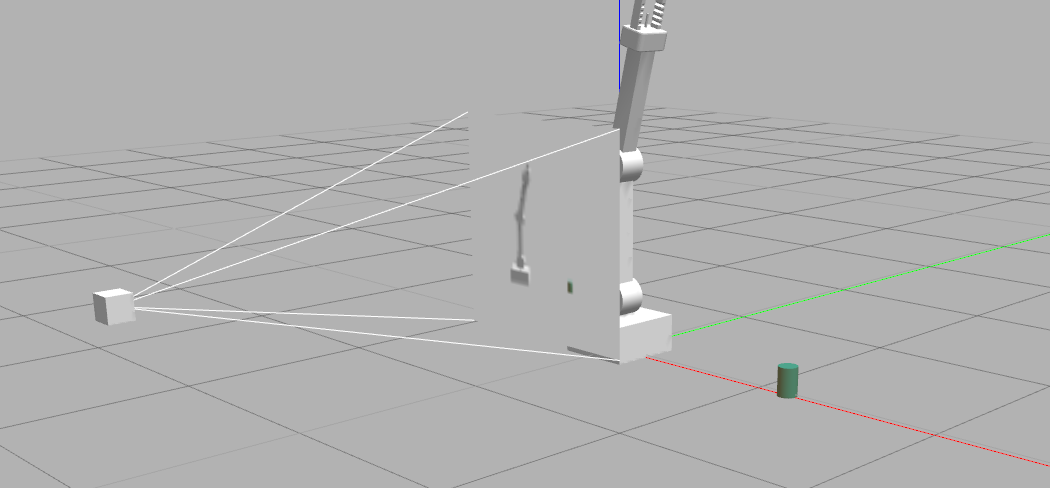
\includegraphics[width=\linewidth]{images/4_training}
      \caption{Simulation setup}
      \label{fig:setup}
\end{figure}

A simulation setup was provided by Udacity was used for the purpose of training the agent (Ref. \ref{fig:setup}).
Camera and collision stream topics are published by the simulation setup which are used to setup the learning algorithm with appropriate reward and penalty function based on the actions taken by the agent. A DQN agent is used for the purpose and position-based control is used for the arm joints.


\subsection{Arm Collision}
The first part of the project was to achieve 90\% accuracy for arm collision with the object in the simulation world.

\begin{figure}[thpb]
      \centering
      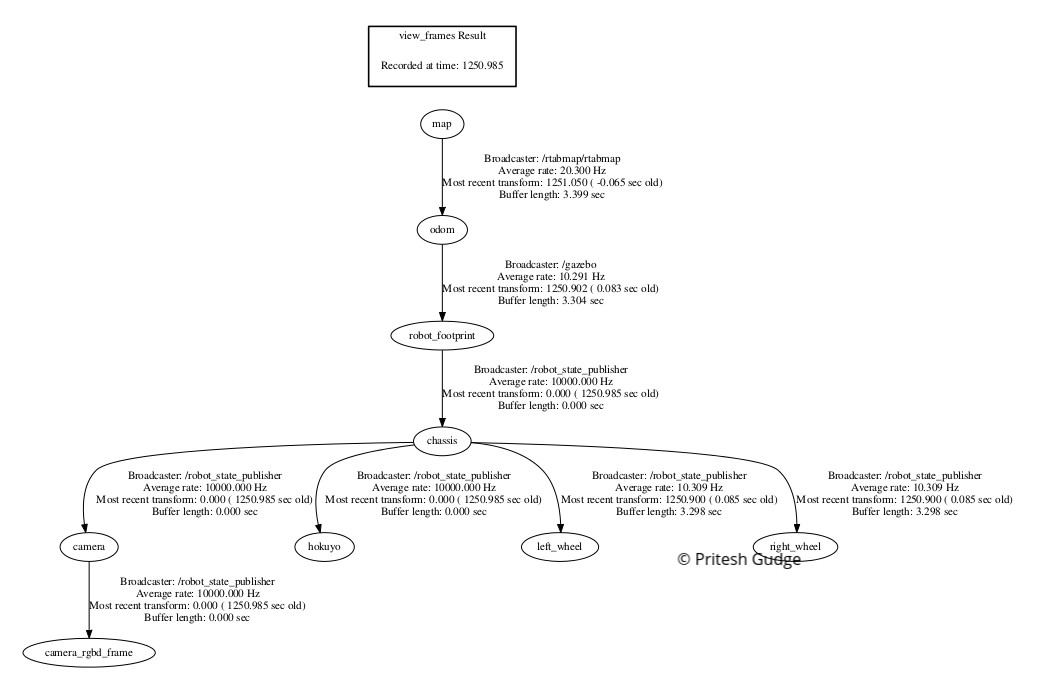
\includegraphics[width=\linewidth]{images/tfframe}
      \caption{TF Frame}
      \label{fig:frame}
\end{figure}

% Robot Models
\subsection{Gripper Collision}
The second part of the project was to achieve 80\% for gripper collision with the object in the simulation world.

\begin{figure}[thpb]
      \centering
      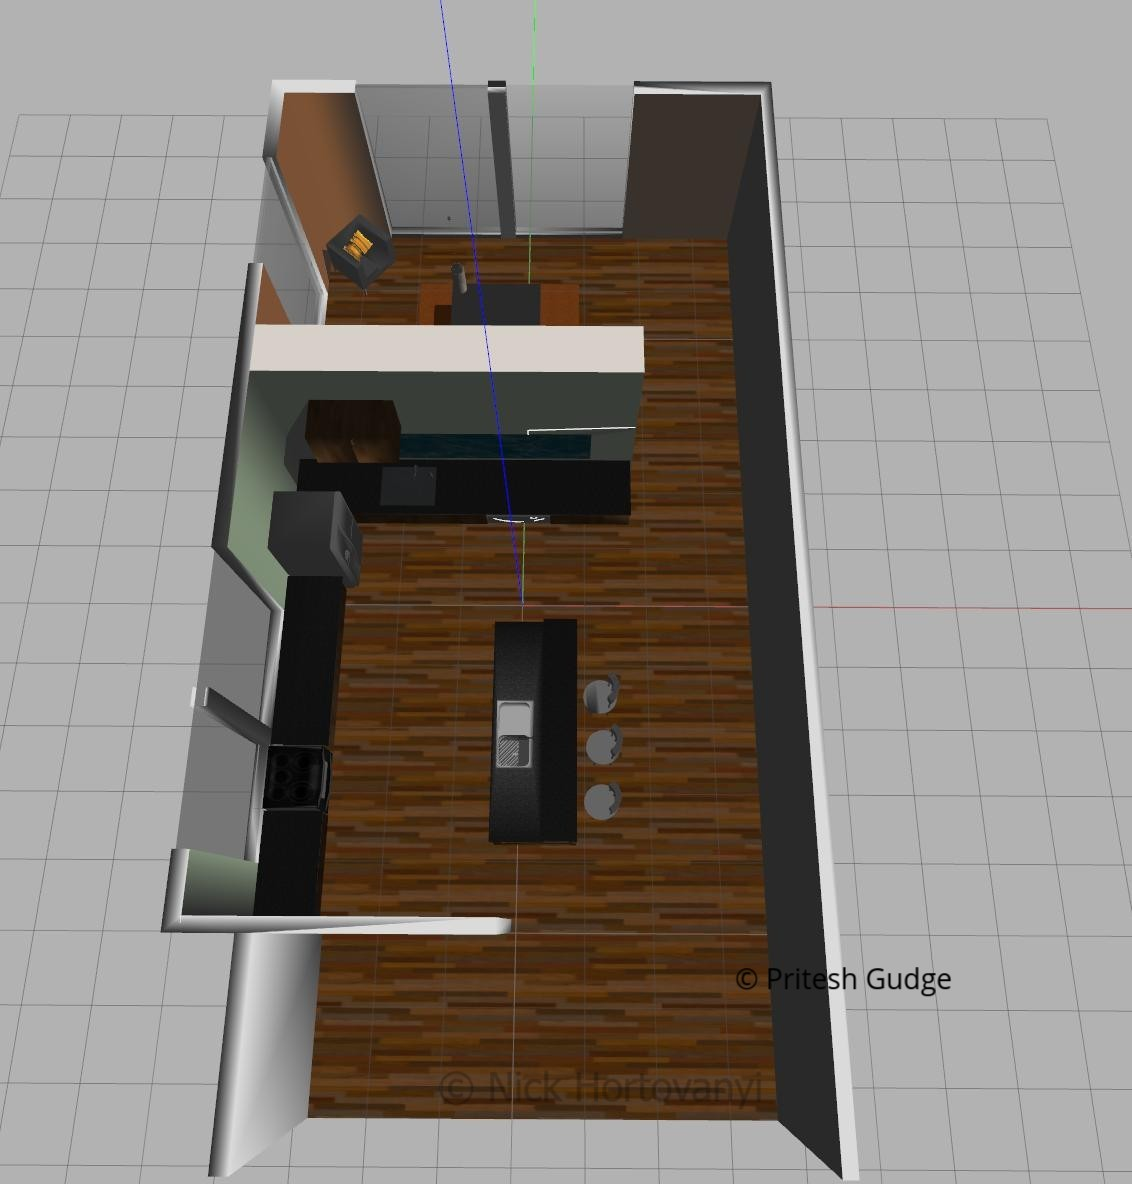
\includegraphics[width=\linewidth]{images/gazebokitchenworld}
      \caption{Kitchen World}
      \label{fig:kitchenworld}
\end{figure}

\begin{figure}[thpb]
      \centering
      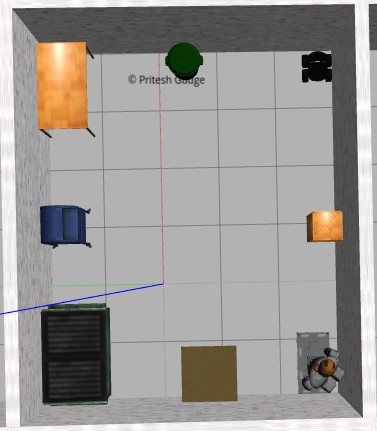
\includegraphics[width=\linewidth]{images/1_world_gz}
      \caption{Custom World}
      \label{fig:customworld}
\end{figure}

\subsubsection{Gripper Collision}
The Kitchen World model was mapped with RtabMap features "Kp/MaxFeatures" 400 and "Vis/MinInliers" at 15, and "Reg/Strategy" 0

The Custom World model was mapped with RtabMap features "Kp/MaxFeatures" 400 and "Vis/MinInliers" at 20, and "Reg/Strategy" 1



\section{Results}

\subsection{Kitchen World}
The kitchen world 2D and 3D maps are shown in figure\ref{fig:kitchen2d} and figure \ref{fig:kitchen3d} respectively. In the 2D Map and the 3D map the general layout of the kitchen and the furniture structures are visible. A total of 198 loop closures were detected(Fig. \ref{fig:kitchenloop}).

\begin{figure}[thpb]
      \centering
      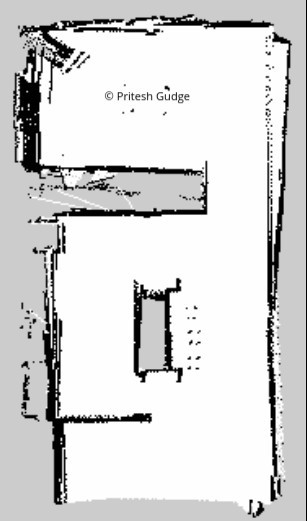
\includegraphics[width=\linewidth]{images/kitchen2dmap}
      \caption{Kitchen World 2D map}
      \label{fig:kitchen2d}
\end{figure}


\begin{figure}[thpb]
      \centering
      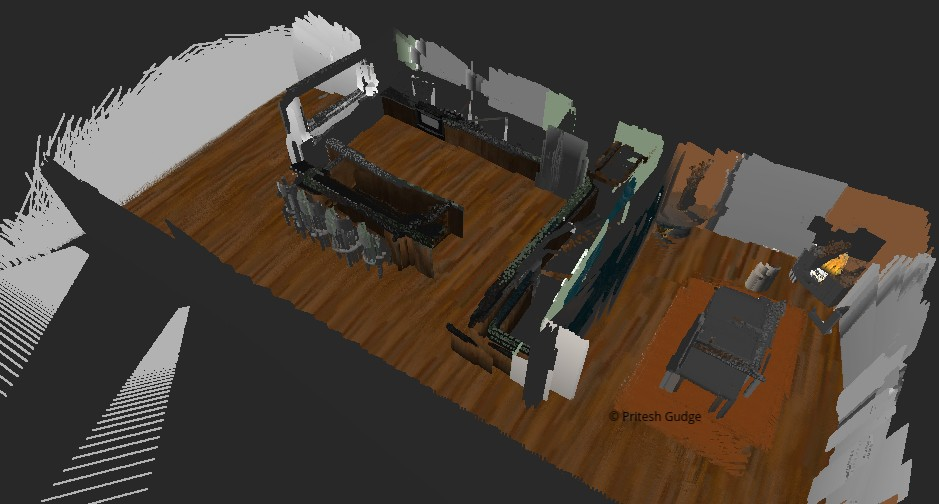
\includegraphics[width=\linewidth]{images/3dmap2}
      \caption{Kitchen World 3D Map}
      \label{fig:kitchen3d}
\end{figure}

\begin{figure}[thpb]
      \centering
      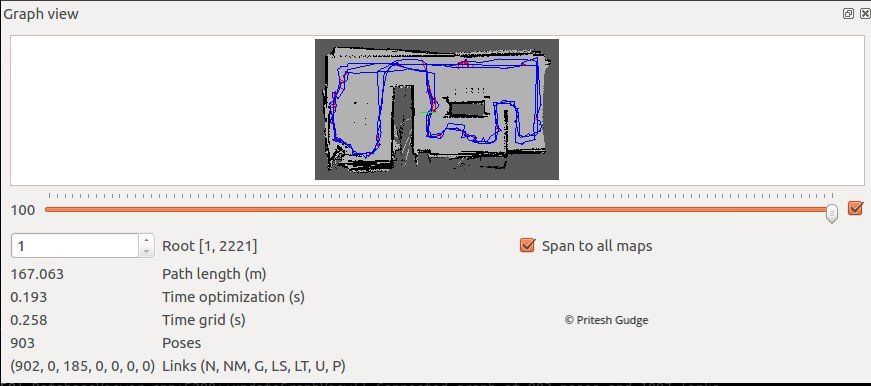
\includegraphics[width=\linewidth]{images/loop_closures}
      \caption{Kitchen World Loop Closures}
      \label{fig:kitchenloop}
\end{figure}

\subsection{Custom World}
The kitchen world 2D and 3D maps are shown in figure\ref{fig:custom2d} and figure \ref{fig:custom3d} respectively. In the 2D Map and the 3D map the general layout of the floor and the furniture structures are visible. A total of 237 loop closures were found(Fig. \ref{fig:customstats} ).

\begin{figure}[thpb]
      \centering
      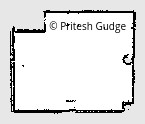
\includegraphics[width=\linewidth]{images/map2_2d}
      \caption{Custom World 2D map}
      \label{fig:custom2d}
\end{figure}


\begin{figure}[thpb]
      \centering
      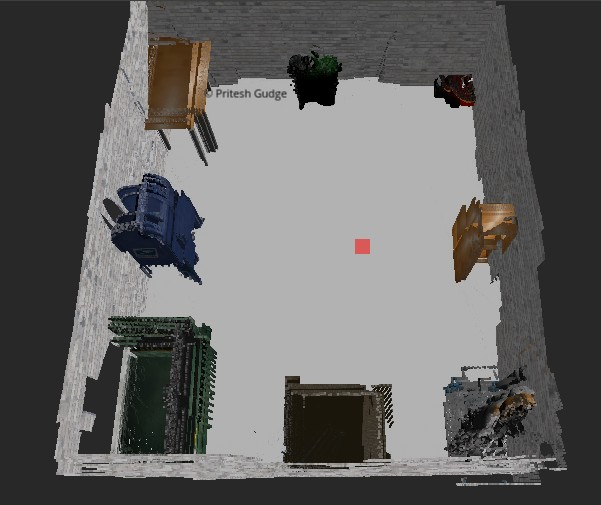
\includegraphics[width=\linewidth]{images/9_3d_view}
      \caption{Custom World 3D Map}
      \label{fig:custom3d}
\end{figure}

\begin{figure}[thpb]
      \centering
      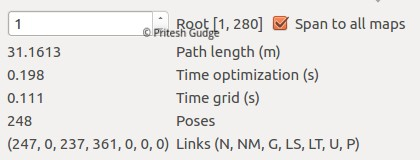
\includegraphics[width=\linewidth]{images/8_graph_stats}
      \caption{Custom World Stats}
      \label{fig:customstats}
\end{figure}
\subsection{Technical Comparison} % only facts
The kitchen\_dining model performed significantly better then the student created cafe model. This was due to the richer and more complex features of the kitchen\_dining model.

\section{Discussion}
The robot was teleoped (navigated via the keyboard) around the room. At some points the robot did not move forward. This appeared to be when it started to perform loop closure. 
The parameters were not changed from the default provided as satisfactory result was obtained with the same.
However the 3D map quickly started to resemble the physical kitchen dining gazebo model. To improve loop detection rates some, on the spot circles were performed. Of particular note were the features in the main kitchen area. More SURF features were identified there as there was more variation in the surfaces.


For the custom layout Vis/MinInliers was increased from 15 to 20 and Reg/Strategy was changed to 1(Including ICP). As the size of the environment was small and to prevent repeated and incorrect loop closures the above values of parameters were chosen.

The custom layout gazebo model wall surfaces were tiled, repeatable pattern with lack of other discerning features sometimes caused the loop closure detection to map to an incorrect previous image. This then distorted the map. Additional features were added to achieve a successful map.



\section{Conclusion / Future work}

Mapping is important to help understand the world. There are a plethora of sensors and of interest is the about to arrive solid state lidars. As the price point of these sensors continues to drop it will open up opportunities to create richer and more realistic 3D maps at a cheaper price point.
Being able to map an environment cost effectively to create a replicated virtual world will increasingly be important to allow for the training of deep learning models. We are actively looking to do this and then supplant the trained model back into a robot so it can navigate in the original environment that was mapped.

\subsection{Modifications for Improvement}
Examples:
\begin{itemize}
\item Adding more sensors to collect data e.g. 3D Lidar
\item Modifying the sensor location and layout. e.g. Adding RGBD camera's to the sides of the robot, to collect data about the lateral surroundings.
\end{itemize}

\subsection{Hardware Deployment}
\begin{enumerate}
\item To be deployed on hardware, a computation unit and appropriate sensors will have to be installed on the robot chassis and the wheels. Proper calibration and verification needs to be done to limit the errors.
\item High CPU and RAM hardware is required to perform SLAM data collection from the multiple sensors, especially to detect loop closures online.
\end{enumerate}



\bibliography{bib}
\bibliographystyle{ieeetr}

\end{document}